\subsection{Session 2, Exercise 7}

\lineparagraph{Exercise}

Give a nondeterministic finite automaton that accepts those words that have 10100 as subword.

\lineparagraph{Solution}

The key to solving this exercise using a nondetermnistic automaton is to create a delayed start on the starting state by introducing a 0,1 loop on it:

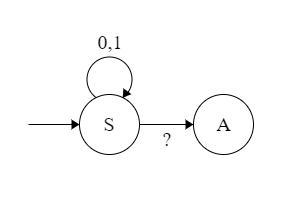
\includegraphics[width=200px]{02/wait_to_start.png}

This will "eat up" some prefix of the input word before allowing the computation to proceed to state A. Whatever we put in place of the ? on the leaving transition will be a nondeterministic choice for the automaton.

The next step is to add the success path to the automaton which contains the string we want to have as a subword: 10100.

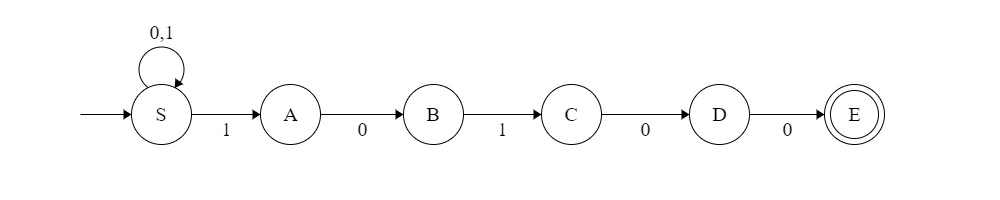
\includegraphics[width=\linewidth]{02/success_path.png}

Then finally, let's allow "eating up" any remaining suffix of the word as well:

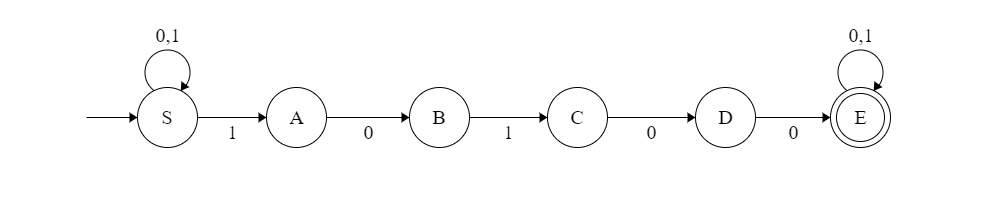
\includegraphics[width=\linewidth]{02/10100.png}

Some observations:

\begin{itemize}
    \item Firstly, this is a nondeterministic finite automaton: Notice how in state $S$, for an input character of $1$ we can either remain in $S$, or move to state $A$.
    \item There are also transitions missing: it is an incomplete finite automaton as well. For example, in state $A$, for an input character of 1, the machine halts (and halting due to a missing transition means rejection, \textbf{regardless of the current state's accept/reject status}.
    \item Notice how visually similar this automaton is to the regular expression for the same language: $(0+1)^*10100(0+1)^*$.
\end{itemize}

Let's look at an example computation on the word 1110100, which is in the language of the automaton.

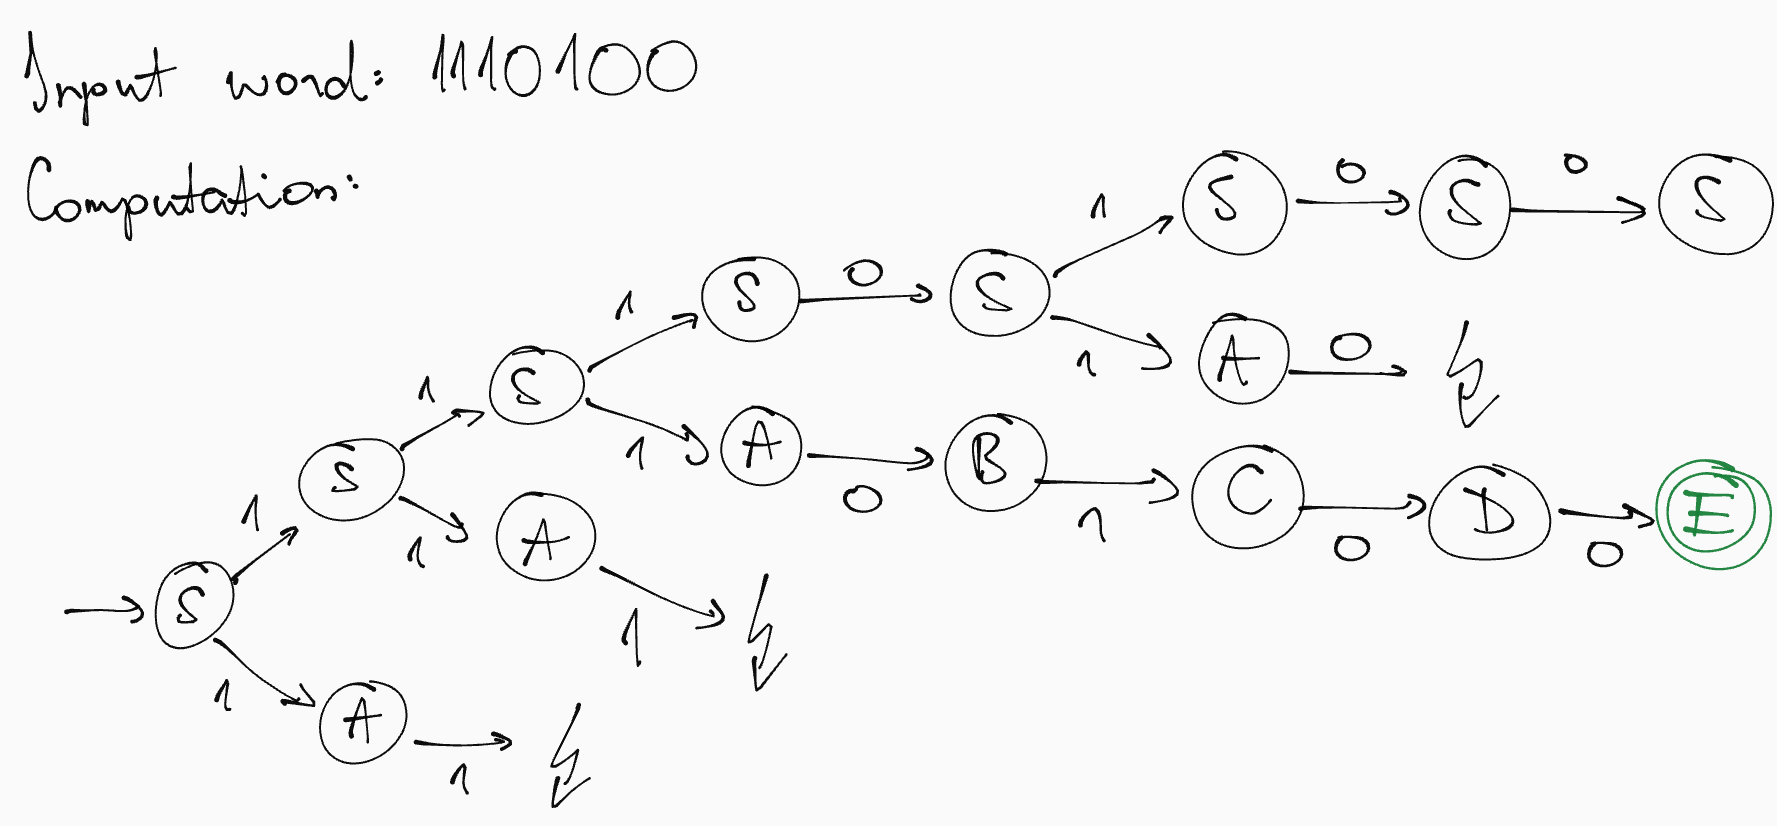
\includegraphics[width=\linewidth]{02/computation_1110100.png}

\begin{itemize}
    \item See, how it tried to leave state $S$ and move to state $A$ many times in different places of the input string? Many times it failed, when the timing was incorrect. Maybe it was too early, when the first two 1's, which are not part of the matching subword were given to it, or it was too late, when the pattern was already gone.
    \item There was already a lazy case, the top branch, which just remained in state $S$ forever, which also could not succeed.
    \item However there only needs to be a single successful branch and it only needs to time its move to state $A$ correctly once: on the third branch it successfully finished in state $E$, which means that the word is accepted, correctly!
    \item Notice how it is only possible to reach state $E$, when the input word contains 10100. We need a 1 to move from $S$ to $A$, then we need a consecutive $0$ to move from $A$ to $B$, then we need a consecutive $1$ to move from $B$ to $C$, then we need a consecutive $0$ to move from $C$ to $D$, then we need another consecutive $0$, to move from $D$ to $E$.
    \item When the timing is just right and we catch the beginning of the pattern we can ''sail smoothly'' towards $E$.
\end{itemize}

When you are on the exam, you will need to give some sort of proof that the automaton you wrote up does what the exercise is asking you to do. For this exercise this is how a proof like this might look like:

\textbf{Proof:}

1. Let's look at the states of the automaton:
What the different states mean and why their transitions are correct.
\begin{itemize}
    \item State $S$ is the starting state. Here, we non-deterministically wait to start our computation, using the $0$,$1$ loop. Since the first character of the pattern we seek is a $1$, on an input character of $1$, the automaton can decide to move to state $A$.
    \item State $A$ represents the information "already read the first character of the pattern". Here, we allow a transition to state $B$ if the second character of the pattern comes, which is a $0$. However, the transition for an input of $1$ is missing, which means that the computation (on that branch) will halt. This is correct, because the pattern's characters must be consecutive.
    \item States $B$, $C$ and $D$ work similaly: they represent the next character recognized from the pattern we seek and we only allow a transition for the upcoming character from the pattern to move forward, towards $E$.
    \item Finally, state $E$ represents "pattern found". This means that we can accept the word, furthermore, any further input characters are allowed, since the pattern can be anywhere in the word.
\end{itemize}

2. Let's look at the accepted and rejected words of the automaton:

Any word that contains the pattern 10100 will be accepted, because the automaton on the (single) accepting branch of the computation first non-deterministically reads the prefix of the word before the pattern, then transitions from $S$, to $E$ using the consecutive characters of the pattern, then finally in state $E$ further characters can be read (the remaining suffix of the word) and the word will be accepted.

Any word that does not contain the pattern 10100 can not reach state $E$, because each step towards $E$ requires the next character of the pattern to be present consecutively in the word. There is correct timing to leave $S$, no computational branch can end up in $E$, so the word will be rejected.

\textbf{(End of proof.)}

(Due to time limits on the exam, it is okay to not use full sentences like I did above, abbreviate things, etc.)

It is important when doing these proofs, that you do not use a specific input word as an example, but generalize to any possible words, like the proof above.

\lineparagraph{Deterministic solution}

This exercise allows us to truly appreciate nondeterministic automata, since it made it really easy for us to come up with a design for a given subword.

However, the task is also possible with a deterministic automaton (it must be, since we can convert any NFA into a DFA, but there is an even easier method to obtain a DFA, than the general conversion algorithm). This is not part of the task, but nice to see how it works as well.

Step 1: Get rid of loop on the starting state, we need to be deterministic now.

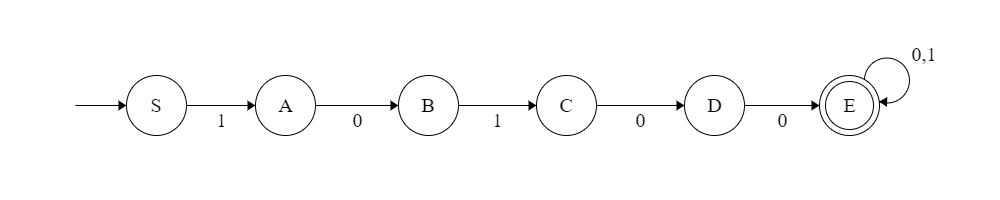
\includegraphics[width=\linewidth]{02/det_10100_1.png}

Step 2: Put in the missing transitions, states $S$-$D$ all miss 1 of them.

The main idea here is that the missing transitions are failures in recognizing the next character of the pattern at the current position. How big of a failure it is depends on what the pattern we have found so far is and how much of it can be salvaged when we add the incorrect character at the end.

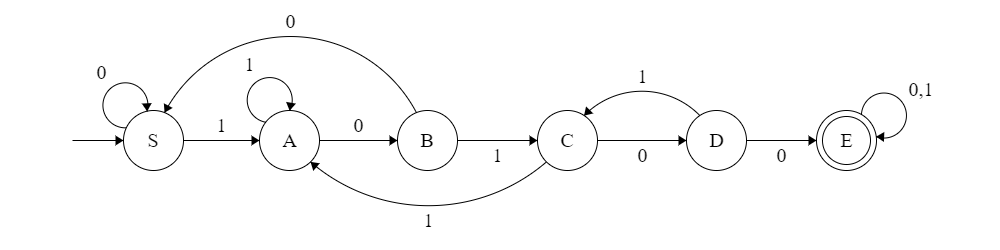
\includegraphics[width=\linewidth]{02/det_10100_2.png}

\begin{itemize}
    \item When we are in state $S$, the pattern we have found so far is nothing. Until we read $0$'s we remain in state $S$, since the first character of the pattern is a $1$.
    \item When we are in state $A$, the pattern we have found so far is ''$1$''. If we read another $1$ now, we now have ''$11$''. The pattern is ''$10100$'', so that second $1$ character can still turn out to be the beginning of the pattern, so we need to remember that we have a ''$1$'' and thus stay in state $A$.
    \item When we are in state $B$, the pattern we have found so far is ''$10$'', if we read a $0$ in now, that makes it a ''$100$''. Unfortunately, there is no salvaging this: not ''$100$'', not ''$00$'' and not even a single ''$0$'' is useful for us, neither of them are the prefixes of the pattern ''$10100$''. We need to scratch everything and go back to state $S$.
    \item When we are in state $C$, the pattern we have found so far is ''$101$''. If we read a $1$ now, that makes it ''$1011$''. The possible suffixes to remember here are ''$011$'', ''$11$'' and ''$1$''. In general we always need to keep the longest one that is still a prefix of the pattern: in this case, that is ''$1$'', which is represented by state $A$, so we move back there.
    \item When we are in state $D$, the pattern we have found so far is ''$1010$''. If we read a $1$ now, that makes it ''$10101$''. This is great news, because we can actually just forget the first two characters and we can still keep the remaining ''$101$'', which is the first three characters of the pattern! Not much is lost, ''$101$'' is represented by state $C$, so we can move there.
\end{itemize}